\section{Methods}\label{sec:methods}

\subsection{Environment}\label{sec:environment}
a basic rundown of the simulation, how it works

\subsubsection{Fire Spread Dynamics}\label{sec:fire_spread}
specifically the fire spread dynamics

\subsubsection{The Reward function}\label{sec:reward_function}
The reward function is a function that maps each state to a value that represents how "good" or desirable that state is. As such, this function is a vital part of the learning process because any reinforcement learning algorithm will rely on two things because they constitute the input to the agent (See basic RL schema). The quality of the state representation, or in other words how much of- and how well the agent sees the environment, and the quality of the reward function, or how well the agents notion of success corresponds with our notion of success and how easy it is to find optima in the reward landscape.

Apart from determining the optimal policy to be learned by the agent, the reward function also determines the speed at which the agent will be able to learn that policy. To take the gradient descent analogy of a problem landscape, if the reward function produces a smooth gradient to the optimal solution, the agent will be able to find a path to that solution more easily than if the reward resembles flat landscape with sparse spikes in which the value jumps from almost always 0 or negative to a positive reward. In other words, the agent should be provided gradual feedback instead of sparse rewards in order to facilitate fast and efficient learning.

Crafting a good reward function for this problem turned out to be quite difficult because it was hard to define a measure of success that is both valid in its formulation and which provides gradual feedback, or a smooth gradient, towards the containment of the fire. We defined the reward function as
\[
R = \left\{\begin{array}{lr}
    1000, & \text{ Fire is contained }\\
    1000 * (p), & \text{ Fire burns out }\\
    -1000, & \text{ Agent dies }\\
    -1 & \text{ Otherwise }

    \end{array}\right\}
\]
where~$p$ is the percent of the map undamaged by either fire or digging. We decided to choose a reward function that defines the goal well, and then compensate for the lack of a smooth gradient with demonstration data to lead it towards the sparse rewards. Note that the 2nd and 3rd states are the only terminal states.

Containment of the fire is determined by (Link to algorithm). The algorithm returns true as soon as it can find a path, not allowing diagonal movements, between any burning cell and any cell on the border of the map. It uses the A* path-finding algorithm to check for a path between any two points.

% Pseudocode for the containment algorithm


\subsubsection{The State Representation}\label{sec:state_rep}
The state of the environment, or the observation of the environment as it is visible to the agent, consists of 3 matrices of size N*M with a boolean domain resulting in, after flattening, an array of (3 * N*M) boolean inputs where (N, M) are the dimensions of the map. Assuming the shape of the map is always square, a map size of (N=10) elements is represented three times: One layer contains only the agent position, translating to a matrix of zeros except for a single one representing the position of the agent. The second layer consists of the position of the fire. Cells that are on fire are represented by a 1, the rest are set to 0. The third layer represents the fire lines cut by the agent in a similar boolean fashion, resulting in a total of 300 inputs to the agent. This is schematically shown in \ref{fig:visiongrid}.

\begin{figure}[h]
    \centering
    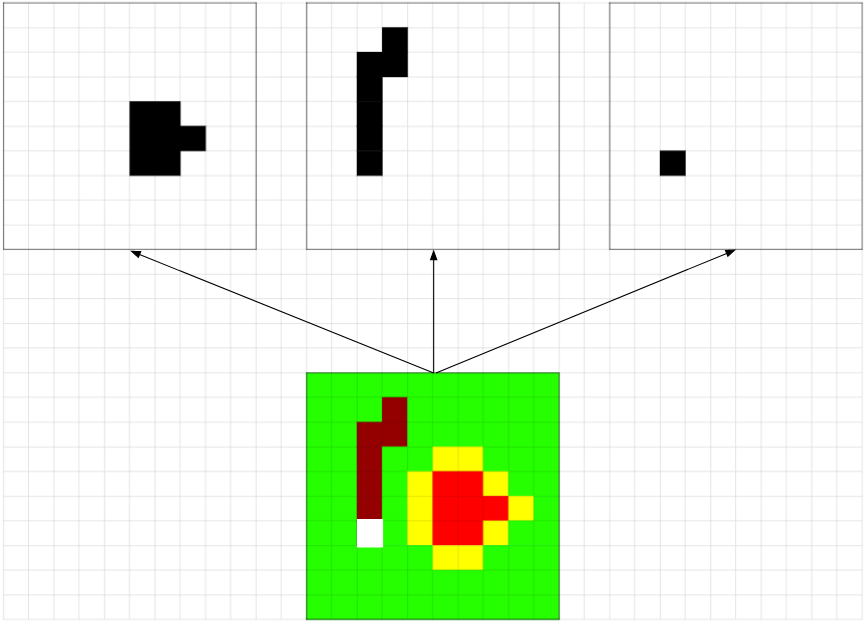
\includegraphics[width=1\linewidth]{img/Vision_Grid.png}
    \caption{A vision grid representation of an example state}
    \label{fig:visiongrid}
\end{figure}

This vision grid approach can speed up the learning process as well as increase the performance (citation Opponent Modelling in the Game of Tron using Reinforcement Learning). Indeed it had a noticeable effect on the performance and learning speed of our implementation compared to a single matrix representing the gray-scaled map as input, likely because the agent can more easily differentiate between different attributes and because only the relevant information is presented. Further, the agent can now see whether the cell it is occupying is already dug or not.


\subsection{The Agent}\label{sec:agent}


\subsubsection{Known Problems with Connectionist RL}\label{sec:problems}
The combination of function approximation (the neural network), bootstrapping (TD methods that update Q-values using estimated return values) and off-policy training (the Q-Learning algorithm) make up the deadly triad \citep{sutton_barto_2018}, which is known to cause instabilities and even divergence in the learning process. There are two well known strategies to reduce this effect and stabilise learning, using experience replay and a target network \citep{mnih2015human}.

\subsubsection{Experience Replay}\label{sec:exp_replay}

\begin{figure}[h]
    \centering
    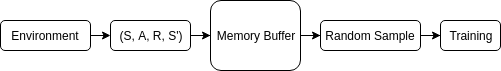
\includegraphics[width=1\linewidth]{img/Experience_Replay.png}
    \caption{Schematic structure of experience replay}
    \label{fig:expreplay}
\end{figure}

Instead of training the network on incoming experiences directly, the experiences can be stored in a memory buffer and the network can be trained on a mini-batch of memories randomly sampled from this buffer (see \ref{fig:expreplay}). This helps because neural networks assume that each training sample is identically and independently distributed with regard to the population the algorithm is set up to approximate (Citation needed), and training directly on incoming experiences break this assumption in two regards.

For one, consecutive incoming experiences are obviously highly correlated because the environment does not radically change after any action (unless it leads to a terminal state). This means that any experience differs from the previous experience only to the extent to which the environment can change in one update step from a single action from the agent. (Citation needed)

The distribution of incoming experiences is also dependent on the agents current policy. If the current policy determines that the agent should head east, then the next experiences recorded by the agent will involve the agent headed east. Apart from the obvious correlation, this can also lead to feedback loops (Explain the loops and cite dqn + paper below)

% https://arxiv.org/pdf/1511.05952.pdf
%(Check out the link for good reasons why experience replay is useful. already in .bib file)

\subsubsection{Target Network}\label{sec:target_network}
Another source of instability is that we use the predictions of the network to generate the target values which, combined with the rest of the update rule which will be explained in the next section, directly update the weights of that same network. This can lead to unwanted feedback loops. We can add a delay to the loop to reduce these effects by using a periodically updated, frozen copy of the network to generate the target values instead (as shown in \ref{fig:targetnet}). Every C iterations, the target network is replaced by a copy of the main network. This modification is called Double Q-Learning \citep{NIPS2010_3964}, and was also used by \citep{mnih2015human} to make the algorithm more stable and prevent divergence.

\begin{figure}[h]
    \centering
    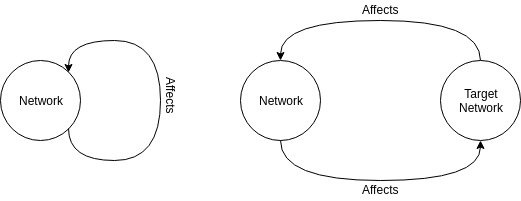
\includegraphics[width=1\linewidth]{img/Target_Network.png}
    \caption{Highlighting the schematic difference of using a target network}
    \label{fig:targetnet}
\end{figure}


\subsubsection{Q-Learning vs SARSA}\label{sec:ql_sarsa}

\subsubsection{Duelling Networks}\label{sec:duelling}

\subsubsection{Demonstration Data}\label{sec:demo_data}
Because the reward function defined earlier provides sparse rewards, the agent needs additional guidance to fast track the learning process. To point it to the right direction, we can fill the memory buffer with human demonstration data before learning. However, this takes a lot of time to do by hand a sufficient number of times and can be automated. To this effect, the pseudocode in (figure so and so) was developed: It randomly picks from a set of two actions which depend on the position of the agent relative to the fire such that the agent will always move in a clockwise motion around the fire. As soon as the containment bonus is collected the environment resets, and this is continued until that bonus has been collected a specified number of times.
% pseudocoooode

\section{The Experimental Setup}\label{sec:experiment}
How were the results collected, which runs were done with which parameters etc

% Insert the algorithm
\begin{algorithm}
  \caption{Baseline algorithm to contain the fire}
  \label{baseline_algo}
  \begin{algorithmic}[1]
    \Procedure{RunBaseline}{}
    \State $totalreward = 0$
    \While {\textbf{not} $done$}
    \State {$action =$ random(possible actions)}
    \If {$action$ is dangerous}
    \State {$action =$ other possible action}
    \EndIf
    \State {$reward, done =$ execute(action)}
    \State $totalreward = totalreward + reward$
    \EndWhile
    \State \Return $totalreward$
    \EndProcedure
  \end{algorithmic}
\end{algorithm}
